%%%%%%%%%%%%%%%%%%%%%%%%%%%%%%%%
%
%
%  Classifying Quaternion Identities
%  (journal article)
%  
%  by Theodore Ehrenborg
%
%
% 
% Last edited: July 19, 2019
%
%
%%%%%%%%%%%%%%%%%%%%%%%%%%%%%%%%%
%
%%%%%%%%%%%%%%%%%%%%%%%%%%%%%%%%%



%%%%%%%%%%%%%%%%%%%%%%%%%%%%%%%%%
%
% pdf settings
%
%%%%%%%%%%%%%%%%%%%%%%%%%%%%%%%%%
%
\pdfpagewidth=8.5truein
\pdfpageheight=11truein





%
%%%%%%%%%%%%%%%%%%%%%%%%%%%%%%%%%



\documentclass[12pt,table]{article}
%\usepackage{anyfontsize}
\usepackage{amssymb, amsmath, fullpage, amsthm}
\usepackage{mathrsfs}
\usepackage{tikz}
\usepackage[title]{appendix}
\usepackage{mathrsfs}
\usepackage{ gensymb }
\usepackage{enumerate}
\usepackage{caption}
\usepackage{comment}
\usepackage{xcolor}
\usepackage{diagbox}
\usepackage[colorinlistoftodos]{todonotes}




\usetikzlibrary{math}
















\parskip2mm

\newtheorem{theorem}{Theorem}[section]
\newtheorem{hypothesis}[theorem]{Hypothesis}
\newtheorem{lemma}[theorem]{Lemma}
\newtheorem{proposition}[theorem]{Proposition}
\newtheorem{corollary}[theorem]{Corollary}
\newtheorem{conjecture}[theorem]{Conjecture}


\theoremstyle{definition}
\newtheorem{definition}[theorem]{Definition}
\newtheorem{example}[theorem]{Example}

\theoremstyle{remark}
\newtheorem{remark}[theorem]{Remark}
\newtheorem{remarks}[theorem]{Remarks}





\hyphenation{Hurwitz}

\font\german = eufm10 scaled\magstep1
\font\Cp = msbm10

\newcommand{\Ccc}{\mathbb C}
\newcommand{\Fff}{\mathbb F}
\newcommand{\Hhh}{\mathbb H}
\newcommand{\Nnn}{\mathbb N}
\newcommand{\Rrr}{\mathbb R}
\newcommand{\Sss}{\mathbb S}
\newcommand{\Zzz}{\mathbb Z}
\newcommand{\Lll}{\mathbb L}
\renewcommand{\Bbb}{\mathbb B}
\newcommand{\Ooo}{\mathbb O}
\newcommand{\Qqq}{\mathbb Q}


\newcommand{\vanish}[1]{}
\newcommand{\coveredby}{\prec}
\newcommand{\divides}{\mid}
\newcommand{\notdivides}{\nmid}
\newcommand{\timesdots}{\times \cdots \times}
\newcommand{\ascodd}{\asc_{\odd}}
\newcommand{\doubleprime}{\prime\prime}
\newcommand{\myfrac}[2]{#1 / #2}
\newcommand{\SSSS}{\mathfrak{S}}
\newcommand{\Gaussian}[2]{\genfrac{[}{]}{0pt}{}{#1}{#2}_q}
\newcommand{\fix}[1]{\todo[inline]{#1}}






\numberwithin{equation}{section}
%\usepackage[bindingoffset=0.2in,
%            left=1in,right=1in,top=1in,bottom=1in,
%            footskip=.25in]{geometry}%Sets margins
%\pagenumbering{gobble}%No page numbers




 


\DeclareMathOperator{\inv}{inv}
\DeclareMathOperator{\frst}{frst}
\DeclareMathOperator{\er}{er}
\DeclareMathOperator{\asc}{asc}
\DeclareMathOperator{\odd}{odd}
\DeclareMathOperator{\Imag}{Im}
\DeclareMathOperator{\Real}{Re}
\DeclareMathOperator{\N}{N}





\begin{document}
%\begin{landscape}


\title{Classifying Quaternion Identities}





\author{\sc Theodore EHRENBORG
\fix{I should thank Professor Leep.}
%\thanks{
%Corresponding author:
%Department of Mathematics,
%University of Kentucky,
%Lexington, KY 40506-0027,
%USA,
%{\tt theodore.ehrenborg@gmail.com}.}
%\:\: 
%\:\:
}



\date{}
%%%\date{Last edited on \today}

\maketitle



\begin{abstract}
This number theory project investigates identities found by
multiplying together quaternions in $ \Lll[x,y,z,w] $, the
Lipschitz quaternions $ \Lll $ adjoined with the
indeterminates $x$, $y$, $z$, $w$.  Recall that quaternions
are $4$-dimensional complex numbers.  These identities provide
solutions to $ \sum_{j = 1}^{p} \tau_j ^ 2 = \left( \sum_{i = 1}^{m}
x_i ^ 2 \right) ^ n $. We present a rigorous definition that captures
the intuitive notion of when two such identities are equivalent. This
definition implies that the true structure of this problem involves the
group action of the direct product $ \mathfrak{S}_4^\pm \times \mathfrak{S}_4^\pm $.  Using
two complementary methods, we compute the number of equivalence
classes for $n = 1, 2, 3, 4,$ where $n$ is the number of
quaternion factors. We move to the case concerning products of complex
numbers, namely $ \Zzz[i][x,y] $. Using the fact that the
Gaussian integers are commutative under multiplication, we
characterize these equivalence classes, thus also providing an
enumeration.
This enumeration quickly gives a proof that
the total number of solutions in $\Zzz[x,y] $
to $a^2 + b^2 = (x^2 + y^2)^n$
is $4n + 4$.
Assuming that all identities when $p = m = 4$
are a product of quaternions, we prove
that
the total number of solutions in $\Zzz[x,y,z,w] $
to $a^2 + b^2 + c^2 + d^2 = (x^2 + y^2 + z^2 + w^2)^n$
is no more than
$ 8 \sum_{i = 0}^n{47^n} $.
Experimental data for $n = 0,1,2,3$
suggests that this expression
is exact.

\end{abstract}

\listoftodos




\section{Introduction}


The author's previous work in~\cite{Ehrenborg_2018}
focused on characterizing the
integer solutions to
$a^2 + b^2 + c^2 + d^2 = e^2$.
This paper explores the polynomial solutions
in $ \Zzz[x,y,z,w] $ to
$a^2 + b^2 + c^2 + d^2 = e^n$, where
$e = x^2 + y^2 + z^2 + w^2$.

In \cite{Ehrenborg_2018} the author characterized integer
solutions by viewing $a^2 + b^2 + c^2 + d^2 = e^2$
as a product of two quaternions. This gave
rise to polynomial solutions to
$a^2 + b^2 + c^2 + d^2 = e^2$
with $e = x^2 + y^2 + z^2 + w^2$.
The paper found that an upper bound for the number
of such solutions is $57$. This paper seeks to
improve that bound, as well as to investigate
the cases when $n > 2$.

\fix{I don't need to mention 57 any more, as I no longer
split up my work every academic year.}

Recall that the \emph{complex numbers} $\Ccc$ are a two-dimensional
field extension of $\Rrr$.
Complex numbers take the form $x + iy$, where $i$ is defined to be the
square root of $-1$ and $x,y \in \Rrr$.
Addition is component-wise, and multiplication
follows from the distributive property and the fact that
$i^2 = -1$.
The \emph{conjugate} of a complex number $ z = x + iy$ is $ \bar{z} = x - iy$, and  
the \emph{norm} is $ \N(z) = z \bar{z} = x^2 + y^2$.  

The \emph{Gaussian integers} $ \Zzz[i] $ are a subring of $\Ccc$:
\[
\Zzz[i] = \{ x + iy: x,y \in \Zzz \}.
\]



Recall that
the \emph{quaternions} $\mathscr{Q}$ are a four-dimensional division ring extension of $\Rrr$.
Quaternions were first discovered by Sir William Rowan Hamilton;
see~\cite{Hamilton}.
Quaternions take the form $x + iy + jz + kw$, with
$x,y,z,w \in \Rrr$, and the linearly independent
elements $i$, $j$, $k$ satisfy the relations:
\begin{align*}
i^2 = j^2 = k^2 = -1,
\\
ij = -ji = k,
\\
jk = -kj = i,
\\
ki = -ik = j.
\end{align*}
Addition is component-wise, and multiplication, which is
in general not commutative,
follows from the distributive property and the preceding relations.
The \emph{conjugate} of a quaternion $ \alpha = x + iy + jz + kw$
is $ \bar{\alpha} = x - iy - jz - kw$,  
and the \emph{norm} is 
$ \N( \alpha ) = \alpha \bar{\alpha} = x^2 + y^2 + z^2 + w^2$.  

The \emph{Lipschitz quaternions} $ \Lll $ are a subring of
the quaternions $\mathscr{Q}$:
\[
\Lll = \{ x + iy + jz + kw \in \mathscr{Q}: x,y,z,w \in \Zzz \}.
\]


In the remainder of this paper $x$, $y$, $z$, $w$ will
usually refer to indeterminates.



The following groups are an essential part of Definition~\ref{def:general}
and Definition~\ref{def:2D}.
\begin{definition}
The {\em symmetric group} $ \mathfrak{S}_n $ is the 
set of all permutations $ \pi = \pi_1 \pi_2 \dotsm \pi_n $ 
of the $ n $ element set $ \{ 1, 2, \dotsc, n \} $,
where $ \pi(i) = \pi_i $.
The {\em signed symmetric group} $ \mathfrak{S}_n^\pm $
is the set of all permutations $ \sigma = \sigma_1 \sigma_2 \dotsm \sigma_n$
of the set $ \{ \pm 1, \pm 2, \dotsc, \pm n \} $ such that
$ | \sigma | = | \sigma_1 | \dotsm |\sigma_n| \in \mathfrak{S}_n $
and $ \sigma(-i) =  -\sigma(i) $.   
\end{definition}



For a signed permutation $ \pi \in \mathfrak{S}_m^\pm $,
let $ \pi $ act on a polynomial in the 
$m$ variables $ x_1,x_2, \dotsc, x_m $ by sending $ x_j $ to 
\[
\pi(x_j) =
\begin{cases}
x_{\pi_j} & \text{if } \pi_j > 0 \\
-x_{-\pi_j} & \text{if } \pi_j < 0
\end{cases}
\]

\begin{definition}
\label{def:general}
Fix $ p, m \in \Nnn $. 
Let $ \tau = ( \tau_1, \tau_2, \dotsc, \tau_p) $
be a tuple of length $ p $ where 
$ \tau_i \in \Zzz[x_1,x_2, \dotsc, x_m] $ for $ i = 1, \dotsc, p $.
We define an equivalence relation, denoted by $ \simeq $, on $p$-tuples
$ \tau $ 
by taking the transitive closure of the following three relations:
\begin{itemize}
\item
$ ( \tau_1, \dotsc, \tau_p) \simeq ( \tau'_1, \dotsc, \tau'_p) $
if there exists a signed permutation $ \pi \in \mathfrak{S}_m^\pm $
acting on the $ m $ variables such that $ \pi( \tau_i ) = \tau'_i $,
 where $ i = 1, \dotsc, p $.
\item
$ ( \tau_1, \dotsc, \tau_p) \simeq ( \tau'_1, \dotsc, \tau'_p) $
if there exists a permutation $ \sigma \in \mathfrak{S}_p $
such that $ \tau_{\sigma(i)} = \tau'_i $, where $ i = 1, \dotsc, p $.
\item
$ ( \tau_1, \dotsc, \tau_p) \simeq ( \pm \tau_1, \dotsc, \pm \tau_p) $
\end{itemize}
\end{definition}


\begin{example}
Definition~\ref{def:general} implies that the following is true:
\begin{align*}
( xz,\: y^2,\: yz )  
&\simeq ( (-y)(-x),\: z^2,\: z(-x) ) \\
&\simeq ( (-y)(-x),\: z(-x),\: z^2 ) \\
&\simeq ( -(-y)(-x),\: z(-x),\: -z^2 ) 
\end{align*}
\end{example}



%Fix $ p \in \Zzz $. 
We are interested in counting the number of
equivalence classes of the set of all tuples
 $ \tau = ( \tau_1, \dotsc, \tau_p) $,
where
%the sum of the squares of the elements of $ \tau $ is
\begin{equation}
\label{equation_general}
\sum_{j = 1}^{p}  \tau_j ^ 2  
= 
\left( \sum_{i = 1}^{m}  x_i ^ 2  \right) ^ n 
\end{equation}
This problem is most easily attacked when we
view $ \left( \sum_{i = 1}^{m}  x_i ^ 2  \right) ^ n $
as the norm of a product of complex numbers or quaternions.
Thus we will focus on the cases where $ p = m = 2 $ and where $ p = m = 4 $.
The general problem can also be viewed as finding the disjoint orbits of 
various tuples, where the group action is $ \mathfrak{S}_p^\pm \times \mathfrak{S}_m^\pm $.



\begin{example}

Consider the case where $ p = m = 2 $ and $ n = 2$.
The following two identities are representatives from 
the two different equivalence classes in this case. These identities
were generated by a product of complex numbers. 

\noindent
Identity I:
\begin{equation*}
(x + iy)(x + iy) = (x^2 - y^2 ) + i(2xy).
\end{equation*}
Taking norms gives the identity
\begin{equation}
\label{eq:Pythagorean}
    (x^2 - y^2 )^2 + (2xy)^2 
    = (x^2 + y^2)^2.
\end{equation}
Identity II:
\begin{equation*}
    (x + iy )(x - iy )
    = (x^2 + y^2 ) + i(0).
\end{equation*}
Taking norms gives the identity
\begin{equation}
    (x^2 + y^2 )^2 + (0)^2
    = (x^2 + y^2 )^2.
\end{equation}
\end{example}

\begin{remark}
Equation~\eqref{eq:Pythagorean} dates back to Euclid; see~\cite{Euclid}. 
\end{remark}

\begin{example}
The following two identities are representatives from 
the two different equivalence classes in the
case where $ p = m = 2 $ and $ n = 3$.
These identities
were generated by a product of complex numbers. 

\noindent
Identity III:
\begin{align*}
    (x + iy)(x + iy)(x + iy) 
    = x(x^2 - 3y^2) + i  y(3x^2 - y^2)  . 
    \end{align*}
Taking norms gives the identity
    \begin{align}
    (x(x^2 - 3y^2))^2 + (  y(3x^2 - y^2) )^2  
    = (x^2 + y^2)^3.
    \end{align}
Identity IV:
    \begin{align*}
    (x + iy )(x + iy)(x - iy ) 
    = x(x^2 + y^2 ) + i(y(x^2 + y^2))  .
    \end{align*}
Taking norms gives the identity
    \begin{align}
    ( x(x^2 + y^2) )^2 + ( y(x^2 + y^2) )^2 
    = (x^2 + y^2 )^3.
    \end{align}
\end{example}







\section{The case where $ p = m = 2$}


In the case where $ p = m = 2$, Definition~\ref{def:general} has an alternate form.



\begin{definition}
\label{def:2D}

Let $ h(z), h'(z) \in \Zzz [i][x,y] $,
where $ z = x + iy $.
Let $ M $ be the following set of mappings: 
\[
M = \{ z \mapsto uz \text{ : } u \in \{ \pm 1, \pm i \} \}  
\cup \{ z\mapsto u \bar{z} \text{ : } u \in \{ \pm 1, \pm i \} \}.  
\]
%Write $ a(x,y) + i \cdot b(x,y) $ and $ a'(x,y) + i \cdot b'(x,y) $ as  $ h(z) $ and  $ h'(z) $, respectively.
We say $ h(z) $ is equivalent to $ h'(z) $,
denoted $ h(z) \simeq h'(z) $,
when there exist mappings $ \varphi, \varphi' \in M $
such that $ \varphi( h( \varphi'( z ) ) )  = h'(z) $.



\end{definition}



\begin{figure}[h]


\begin{center}
\begin{tikzpicture}

\tikzmath{
\scale = .7;
}


\draw[thick] (-5*\scale,0) -- (5*\scale,0);
\draw[thick] (0,-5*\scale) -- (0,5*\scale);

\fill (2 * \scale , 4*\scale) circle (0.1*\scale) node[anchor=east] {\Large $ z $ };
\fill (4 * \scale , -2*\scale) circle (0.1*\scale) node[anchor=west] {\Large $ -iz $ };
\fill (-2 * \scale , -4*\scale) circle (0.1*\scale) node[anchor=west] {\Large $ -z $ };
\fill (-4 * \scale , 2*\scale) circle (0.1*\scale) node[anchor=east] {\Large $ iz $ };

\fill (2 * \scale , -4*\scale) circle (0.1*\scale) node[anchor=east] {\Large $ \bar{z} $ };
\fill (4 * \scale , 2*\scale) circle (0.1*\scale) node[anchor=west] {\Large $ i\bar{z} $ };
\fill (-2 * \scale , 4*\scale) circle (0.1*\scale) node[anchor=west] {\Large $ -\bar{z} $ };
\fill (-4 * \scale , -2*\scale) circle (0.1*\scale) node[anchor=east] {\Large $ -i\bar{z} $ };

  

\end{tikzpicture}

\end{center}

\caption{
The set $M$ in Definition~\ref{def:2D} is isomorphic to
the signed symmetric group $ \mathfrak{S}_2^\pm $.
}
 
\label{fig:2D_transformations}
 
\end{figure}



\begin{lemma}
The relation $ \simeq $ is an equivalence relation.
\end{lemma}

\begin{proof}
The relation $ \simeq $ satisfies the three conditions of an equivalence relation:
\begin{enumerate}
\item Reflexive Property: If we choose $ \mu $ and $ \mu'$ to be the identity map $ z \mapsto z $, 
then $ h(z) \simeq h(z) $.

\item Symmetric Property: Let  $ h(z) \simeq h'(z) $, that is, there exist mappings 
$ \mu, \mu' \in M $
such that $ \mu( h( \mu'( z ) ) )  = h'(z) $.
The set $M$ is isomorphic to the signed symmetric group $ \mathfrak{S}_2^\pm $,
so every mapping in $M$
has an inverse in $M$. As  $ \mu^{-1}( h'( (\mu')^{-1}( z ) ) )  = h(z) $,
we have $ h'(z) \simeq h(z) $.

\item Transitive Property: Let $ a(z) \simeq b(z) $ and $ b(z) \simeq c(z) $. By the 
Symmetric Property, we have $ c(z) \simeq b(z) $. Thus there exist mappings
$ \mu, \mu', \nu, \nu' \in M $ such that $ \mu( a( \mu'( z ) ) )  = b(z) $ and 
$ \nu( c( \nu'( z ) ) )  = b(z) $. As a result we obtain
\[
\mu( a( \mu'( z ) ) ) = \nu( c( \nu'( z ) ) ). 
\]
Thus we have
\[
a(  z  ) = \mu^{-1}( \nu( c( (\mu')^{-1}( \nu'( z ) ) ) ) ).
\]
This means that $ c(z) \simeq a(z) $ or $ a(z) \simeq c(z) $. \qedhere
\end{enumerate}
\end{proof}

Recall that given $ a(x,y), b(x,y) \in \Zzz[x,y] $,
we can find $ h(z) \in \Zzz [i][x,y] $
such that
$ z = x + iy $
and
$ h(z) = a(x,y) + i \cdot b(x,y) $. 
The converse is also true.



\begin{lemma}
Let $ h(z) \simeq h'(z) $, where $ h(z), h'(z) \in \Zzz[i][x,y] $
and $ z = x+ iy $.
Suppose $ ( x^2 + y^2 ) ^ u \divides h(z) $,
where $ u \in \Nnn $. Then $ ( x^2 + y^2 ) ^ u \divides h'(z) $ also holds.
\end{lemma}
   
\begin{proof}
Let $ h(z) = ( x^2 + y^2 ) ^ u  p(z) $, where $ p(z) \in \Zzz [i][x,y] $. 
Whatever mappings we apply to $h$ and $z$
to obtain $ h'(z) $, we also apply to the factors of $ h(z) $. 
No mapping will remove the factor of $ ( x^2 + y^2 ) ^ u $.
\end{proof}

\vanish{
\begin{corollary}
Let $ h(z), h'(z) \in \Zzz[i][x,y] $ with $ z = x+ iy $.
\[
h(z) \simeq h'(z) 
\implies 
( \forall u \in \Nnn \cup \{ 0 \},  ( x^2 + y^2 ) ^ u \divides h(z)  \iff ( x^2 + y^2 ) ^ u \divides h'(z)  )
\]
\end{corollary}
}

\begin{corollary}
\label{corollary_equivalence}
Let $ h(z), h'(z) \in \Zzz[i][x,y] $ with $ z = x+ iy $.
Suppose $ h(z) \simeq h'(z) $. Then for all  $ u \in \Nnn \cup \{ 0 \} $,
the following two conditions are
equivalent:
\begin{enumerate}[i.]
\item $ ( x^2 + y^2 ) ^ u \divides h(z) $,
\item $ ( x^2 + y^2 ) ^ u \divides h'(z) $.
\end{enumerate}
\end{corollary}



\begin{theorem}
\label{thm:2D_equivalence}
Consider the set of all $2$-tuples $ \tau = ( \tau_1, \tau_2 )$ where 
$
  \tau_1 ^ 2   +   \tau_2 ^ 2   
= 
\left(  x_1 ^ 2 + x_2 ^ 2  \right) ^ n 
$.
The number of equivalence classes within this set 
is exactly  $ \left\lfloor \myfrac{n}{2} \right\rfloor + 1 $. 
Moreover, each equivalence class contains a tuple
of the form $ ( \Real( \beta ) , \Imag( \beta ) ) $,
where $ \beta = (x + iy)^j (x -  iy)^{n-j} $,
with $ j $
being one of $ 0, 1, \dotsc, \left\lfloor \myfrac{n}{2} \right\rfloor $.
\end{theorem}
%Should I include a section about Professor Leep's extension of
%this result?
%
%I don't think so. He would then become a coauthor, and it's hard to
%do a long-distance collaboration.
\begin{proof}
Suppose 
\[
(x^2 + y^2)^n = a(x,y)^2 + b(x,y)^2,
\]
where $ a(x,y), b(x,y) \in \Zzz[x,y] $.
Both sides of the equation can be factored, leading to  
\[
(x + iy)^n (x -  iy)^n = ( a(x,y) + i \cdot b(x,y) ) ( a(x,y) - i \cdot b(x,y) ) .
\]
Since $ \Zzz [i][x,y] $ is a unique factorization domain,
we can factor this as
\[
a(x,y) + i \cdot b(x,y) = c \cdot (x + iy)^j (x -  iy)^k
\]
and
\[
a(x,y) - i \cdot b(x,y) = d \cdot (x + iy)^r (x -  iy)^s,
\]
where $ j, k, r, s \in \Nnn \cup \{0\} $ and
$c \cdot d = 1 $ with $ c,d \in \{ \pm 1 , \pm i \} $. 
We know $ j + r = n $ and $ k + s = n $, as well as
(by taking norms) $ j + k = n $ and $ r + s = n $.
Thus $k = r$ and $j = s$.

Clearly the relation
$ a(x,y) + i \cdot b(x,y) \simeq  a(x,y) - i \cdot b(x,y) $
holds.
Since 
\[ 
a(x,y) + i \cdot b(x,y) = c \cdot (x + iy)^j (x -  iy)^{n-j} 
\]
and 
\[ 
a(x,y) - i \cdot b(x,y) = d \cdot (x + iy)^{n-j} (x -  iy)^j,
\]
each equivalence class contains a representative with $ j \leq n - j
$.  As $ 2j \leq n $, we have $ j \leq \myfrac{n}{2} $, so $ j $
is one of $ 0, 1, \dotsc, \left\lfloor \myfrac{n}{2} \right\rfloor $. This shows
that there are at most $ \left\lfloor \myfrac{n}{2} \right\rfloor + 1 $
equivalence classes. Now we show that there are at least that many.



Consider $ (x + iy)^u (x -  iy)^{n-u} $  and $ (x + iy)^v (x -  iy)^{n-v} $,
where $ u \neq v $ and $u,v \leq \left \lfloor \myfrac{n}{2} \right \rfloor $. We have
\begin{align*}
(x + iy)^u (x -  iy)^{n-u} &= (x^2 + y^2)^u (x -  iy)^{n-2u},
\\
(x + iy)^v (x -  iy)^{n-v} &= (x^2 + y^2)^v (x -  iy)^{n-2v}.
\end{align*}
Without loss of generality, we may assume $ u > v $. 
Since $ \Zzz [i][x,y] $ is a unique factorization domain,
$ (x^2 + y^2) \notdivides (x -  iy)^e $ for $ e \in \Nnn \cup \{ 0 \} $.
Thus $ (x^2 + y^2)^u \divides (x + iy)^u (x -  iy)^{n-u} $
but $ (x^2 + y^2)^u \notdivides (x + iy)^v (x -  iy)^{n-v} $.

By Corollary~\ref{corollary_equivalence},
$ (x + iy)^u (x -  iy)^{n-u} \not\simeq (x + iy)^v (x -  iy)^{n-v} $, 
so the $ \left\lfloor \myfrac{n}{2} \right\rfloor + 1 $ representatives arise from
distinct equivalence classes.
Thus there are $ \left\lfloor \myfrac{n}{2} \right\rfloor + 1 $ equivalence classes, 
one each for $ u = 0, 1, \dotsc,  \left\lfloor \myfrac{n}{2} \right\rfloor $.
\end{proof}







\begin{figure}[h]


\begin{center}
\begin{tikzpicture}

\tikzmath{
\hash = 0.1;
\height = 6;
\length = 10;
\scale = 1;
}


\draw[thick] (0,0) -- (\scale * \length,0);
\fill (\scale * \length/2, -1) circle (0cm) node[anchor=north] {\Large $ n $ };

\draw[thick] (0,0) -- (0,\scale * \height);
%\fill (-2, \scale * \height/2 ) circle (0cm) node[rotate=90,anchor=south] {\Large  Number of };
%\fill (-1, \scale * \height/2 ) circle (0cm) node[rotate=90,anchor=south] {\Large  equivalence classes };
\fill (-1, \scale * \height/2 ) circle (0cm) node[anchor=east] {\Large  $ \kappa $ };


\foreach \y in {1, ..., \height}
    \draw[thick] ( -\hash, \scale * \y ) node[anchor=east] {\Large \y} -- ( \hash, \scale * \y );

\foreach \x in {1, ..., \length}
{
   \draw[thick] ( \scale * \x, -\hash ) node[anchor=north] {\Large \x} -- ( \scale * \x, \hash ) ;
   \fill (\scale * \x, { \scale *  floor( \x / 2 ) + \scale } ) circle (\scale * .1cm);
}
  

\end{tikzpicture}

\end{center}

\caption{
The number of equivalence classes $ \kappa $
when $p = m = 2$ is $ \left\lfloor \myfrac{n}{2} \right\rfloor + 1 $ .
 }
 
\label{fig:2D}
 
\end{figure}



\begin{corollary}

The number of solutions $ (a, b) $ to
\[
a^2 + b^2 = (x^2 + y^2)^n,
\]
where $ a, b \in \Zzz[x,y] $, is $4n + 4$.

\end{corollary}
\begin{proof}
It is sufficient to count the orbits of a representative from each
equivalence class, where the group action is
$ \mathfrak{S}_2^\pm \times \mathfrak{S}_2^\pm $.

\noindent
Case I: $ n = 2z $ for some $ z \in \Zzz $.

There are $ z + 1 $ equivalence classes. We choose $ z + 1 $
representatives of the form $ (x - iy)^j (x + iy)^k $, with
$ 0 \leq j \leq \myfrac{n}{2}$ and $ j + k = n $.
When $ j = k $, the representative
is $ (x - iy)^z (x + iy)^z = ( x^2 + y^2 ) ^ z $.
This gives the tuple $ ( x^2 + y^2, 0 ) $, which has an orbit of order 4.
Otherwise, we write the representative as $ (x + iy)^{k-j} (x^2 + y^2)^j $.
As $ k - j $ is even, let $ k - j = 2w $. We have
\begin{align}
\label{equation_first_binomial}
(x + iy) ^ {2w} &= x ^ {2w} - \binom{2w}{2}  x^{2w - 2 } y^2
+ \dotsb + \binom{2w}{2w-2} x^2 y^{2w - 2} (-1) ^ {w - 1}
+  y^{2w} (-1) ^ {w} \nonumber
\\
&+ i \left( \binom{2w}{1} x ^ {2w - 1} y + \dotsb +
\binom{2w}{2w-1}  x y ^ {2w -1} (-1)^{w-1} \right).
\end{align}
As a tuple, this has two entries, where the first is the real part
of equation~\eqref{equation_first_binomial} and the second entry
is the imaginary part.
The order of the stabilizer is 8 --- the two variables can be rearranged and their
signs switched. This may require the sign of an entire expression to be switched,
depending on the parity of $ w $.
As $ | \mathfrak{S}_2^\pm \times \mathfrak{S}_2^\pm | = 64$, the order of each orbit
is also 8. 

Thus in Case I there are $ 8z + 4 = 4 (n + 1 ) $ solutions
to $ a^2 + b^2 = (x^2 + y^2)^n $.



\noindent
Case II: $ n = 2z + 1$ for some $ z \in \Zzz $.

There are $ z + 1 $ equivalence classes. We choose $ z + 1 $
representatives of the form $ (x - iy)^j (x + iy)^k $, with
$ 0 \leq j \leq \myfrac{n}{2}$ and $ j + k = n $.
It is impossible to
choose $ j $ such that $ \Imag\left( (x - iy)^j (x + iy)^k \right) = 0$.
We write the representative as $ (x + iy)^{k-j} (x^2 + y^2)^j $.
As $ k - j $ is odd, let $ k - j = 2w + 1 $. We have
\begin{align}
\label{equation_second_binomial}
(x + iy) ^ {2w + 1} &= x ^ {2w + 1} - \binom{2w+1}{2}  x^{2w - 1 } y^2
+ \dotsb + \binom{2w+1}{2w} x y^{2w} (-1) ^ {w} \nonumber
\\
&+ i \left( \binom{2w+1}{1} x ^ {2w} y + \dotsb +
\binom{2w+1}{2w-1}  x^2 y ^ {2w -1} (-1)^{w-1}
+  y^{2w+1} (-1) ^ {w}
\right).
\end{align}
As a tuple, this has two entries, where the first is the real part
of equation~\eqref{equation_second_binomial} and the second entry
is the imaginary part.
The order of the orbit of the tuple under the group action is 8, which can be
verified in a similar manner to Case I.

Thus the number of solutions in Case II is $ 8(z + 1) = 4 ( 2w + 1) + 4 = 4n + 4 $.
\end{proof}




\section{The case where $p = m = 4$}
\label{sec:4D}

In this section we examine the case where
$p = m = 4$ in equation~\eqref{equation_general}.
This case is approached by factoring the identities
into quaternions in $\Lll[x,y,z,w]$. The quaternions'
lack of multiplicative commutativity precludes the 
technique used in the proof of Theorem~\ref{thm:2D_equivalence},
so experimental data becomes more important.


Two methods of gathering experimental data about the 
number of equivalence classes are used. 
In the first method,
the program \emph{numeric\_comparison}
is used to calculate specific numerical values of 
the identities in order to 
separate them into equivalence classes.
If two identities fulfill
a different set of solutions, they are
not equivalent.




\begin{table}[t]



\begin{center}


\begin{tabular}{ r || c | c | c | c | c | c | c | c | }
\diagbox{Value}{Identity} & \eqref{Identity_1} & \eqref{Identity_2}
& \eqref{Identity_3} & \eqref{Identity_4}
& \eqref{Identity_5} & \eqref{Identity_6}
& \eqref{Identity_7} & \eqref{Identity_8}
\\
\hline\hline
$0^2 + 0^2 + 0^2 + 0^2 = 0^2$ & \cellcolor{gray!50} & \cellcolor{gray!50}
& \cellcolor{gray!50} & \cellcolor{gray!50}
& \cellcolor{gray!50} & \cellcolor{gray!50}
& \cellcolor{gray!50} & \cellcolor{gray!50}
\\
\hline
$0^2 + 0^2 + 0^2 + 1^2 = 1^2$ & \cellcolor{gray!50} & \cellcolor{gray!50}
& \cellcolor{gray!50} & \cellcolor{gray!50}
& \cellcolor{gray!50} & \cellcolor{gray!50}
& \cellcolor{gray!50} & \cellcolor{gray!50}
\\
\hline
$0^2 + 0^2 + 0^2 + 2^2 = 2^2$ & \cellcolor{gray!50} & \cellcolor{gray!50}
& \cellcolor{gray!50} & \cellcolor{gray!50}
& \cellcolor{gray!50} & \cellcolor{gray!50}
& \cellcolor{gray!0} & \cellcolor{gray!0}
\\
\hline
$0^2 + 0^2 + 0^2 + 3^2 = 3^2$ & \cellcolor{gray!50} & \cellcolor{gray!0}
& \cellcolor{gray!50} & \cellcolor{gray!50}
& \cellcolor{gray!50} & \cellcolor{gray!0}
& \cellcolor{gray!50} & \cellcolor{gray!50}
\\
\hline
$0^2 + 0^2 + 0^2 + 4^2 = 4^2$ & \cellcolor{gray!0} & \cellcolor{gray!50}
& \cellcolor{gray!50} & \cellcolor{gray!0}
& \cellcolor{gray!50} & \cellcolor{gray!0}
& \cellcolor{gray!0} & \cellcolor{gray!50}
\\
\hline
$0^2 + 1^2 + 2^2 + 2^2 = 3^2$ & \cellcolor{gray!50} & \cellcolor{gray!50}
& \cellcolor{gray!0} & \cellcolor{gray!50}
& \cellcolor{gray!50} & \cellcolor{gray!50}
& \cellcolor{gray!50} & \cellcolor{gray!50}
\\
\hline
$1^2 + 1^2 + 1^2 + 1^2 = 2^2$ & \cellcolor{gray!0} & \cellcolor{gray!0}
& \cellcolor{gray!0} & \cellcolor{gray!50}
& \cellcolor{gray!50} & \cellcolor{gray!50}
& \cellcolor{gray!50} & \cellcolor{gray!50}
\\
\hline
$2^2 + 2^2 + 2^2 + 2^2 = 4^2$ & \cellcolor{gray!50} & \cellcolor{gray!0}
& \cellcolor{gray!0} & \cellcolor{gray!50}
& \cellcolor{gray!0} & \cellcolor{gray!50}
& \cellcolor{gray!50} & \cellcolor{gray!0}
\\
\hline
\end{tabular}





\end{center}
\caption{
Small data values used by
\emph{numeric\_comparison}
to differentiate between equivalence classes
of identities. 
Shaded cells indicate that the particular value
of $ a^2 + b^2 + c^2 + d^2 = e^2$ was a particular
value of the identity.
}

\label{table_barcode}


\end{table}

For $n = 2$, a sample of this process
appears in Table~\ref{table_barcode}.
This program provides a lower
bound on the number of identities, but 
cannot prove that two identities are 
equivalent.

\begin{figure}[h]


\begin{center}
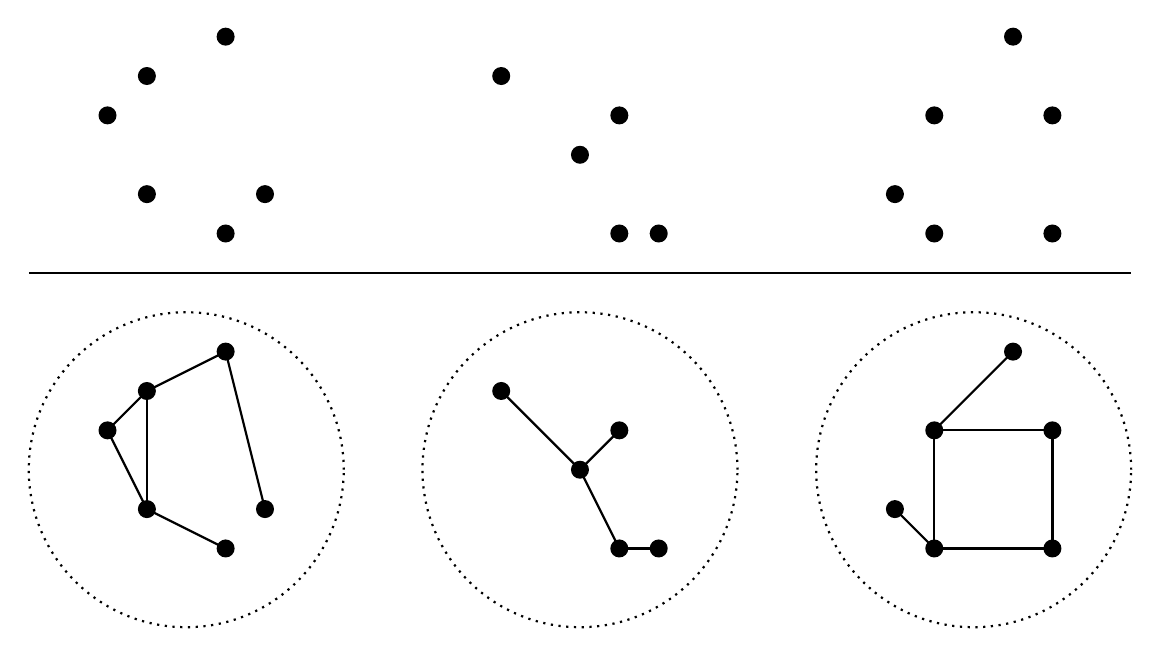
\begin{tikzpicture}

\tikzmath{
\scale = 1;
}

\draw[thick,dotted] (0*\scale,0*\scale) circle(2*\scale);
\draw[thick,fill] (0*\scale,0*\scale) circle(0.1*\scale);
\draw[thick,fill] (0.5*\scale,0.5*\scale) circle(0.1*\scale);
\draw[thick,fill] (-1*\scale,1*\scale) circle(0.1*\scale);
\draw[thick,fill] (0.5*\scale,-1*\scale) circle(0.1*\scale);
\draw[thick,fill] (1*\scale,-1*\scale) circle(0.1*\scale);
\draw[thick] (0*\scale,0*\scale) -- (.5*\scale,.5*\scale);
\draw[thick] (0*\scale,0*\scale) -- (.5*\scale,-1*\scale);
\draw[thick] (.5*\scale,-1*\scale) -- (1*\scale,-1*\scale);
\draw[thick] (0*\scale,0*\scale) -- (-1*\scale,1*\scale);


\draw[thick,dotted] (5*\scale,0*\scale) circle(2*\scale);
\draw[thick,fill] (6*\scale,.5*\scale) circle(0.1*\scale);
\draw[thick,fill] (5.5*\scale,1.5*\scale) circle(0.1*\scale);
\draw[thick,fill] (4.5*\scale,.5*\scale) circle(0.1*\scale);
\draw[thick,fill] (4*\scale,-.5*\scale) circle(0.1*\scale);
\draw[thick,fill] (4.5*\scale,-1*\scale) circle(0.1*\scale);
\draw[thick,fill] (6*\scale,-1*\scale) circle(0.1*\scale);
\draw[thick] (6*\scale,.5*\scale) -- (4.5*\scale,.5*\scale);
\draw[thick] (5.5*\scale,1.5*\scale) -- (4.5*\scale,.5*\scale);
\draw[thick] (6*\scale,-1*\scale) -- (4.5*\scale,-1*\scale);
\draw[thick] (4.5*\scale,-1*\scale) -- (4*\scale,-.5*\scale);
\draw[thick] (4.5*\scale,.5*\scale) -- (4.5*\scale,-1*\scale);
\draw[thick] (6*\scale,-1*\scale) -- (6*\scale,.5*\scale);





\draw[thick,dotted] (-5*\scale,0*\scale) circle(2*\scale);
\draw[thick,fill] (-4.5*\scale,1.5*\scale) circle(0.1*\scale);
\draw[thick,fill] (-5.5*\scale,1*\scale) circle(0.1*\scale);
\draw[thick,fill] (-6*\scale,.5*\scale) circle(0.1*\scale);
\draw[thick,fill] (-5.5*\scale,-.5*\scale) circle(0.1*\scale);
\draw[thick,fill] (-4.5*\scale,-1*\scale) circle(0.1*\scale);
\draw[thick,fill] (-4*\scale,-.5*\scale) circle(0.1*\scale);
\draw[thick] (-4.5*\scale,-1*\scale) -- (-5.5*\scale,-.5*\scale);
\draw[thick] (-5.5*\scale,1*\scale) -- (-5.5*\scale,-.5*\scale);
\draw[thick] (-5.5*\scale,-.5*\scale) -- (-6*\scale,.5*\scale);
\draw[thick] (-6*\scale,.5*\scale) -- (-5.5*\scale,1*\scale);
\draw[thick] (-5.5*\scale,1*\scale) -- (-4.5*\scale,1.5*\scale);
\draw[thick] (-4*\scale,-.5*\scale) -- (-4.5*\scale,1.5*\scale);


\draw[thick] (-7*\scale,2.5*\scale) -- (7*\scale,2.5*\scale);


\draw[thick,fill] (0*\scale,4*\scale) circle(0.1*\scale);
\draw[thick,fill] (0.5*\scale,4.5*\scale) circle(0.1*\scale);
\draw[thick,fill] (-1*\scale,5*\scale) circle(0.1*\scale);
\draw[thick,fill] (0.5*\scale,3*\scale) circle(0.1*\scale);
\draw[thick,fill] (1*\scale,3*\scale) circle(0.1*\scale);




\draw[thick,fill] (6*\scale,4.5*\scale) circle(0.1*\scale);
\draw[thick,fill] (5.5*\scale,5.5*\scale) circle(0.1*\scale);
\draw[thick,fill] (4.5*\scale,4.5*\scale) circle(0.1*\scale);
\draw[thick,fill] (4*\scale,3.5*\scale) circle(0.1*\scale);
\draw[thick,fill] (4.5*\scale,3*\scale) circle(0.1*\scale);
\draw[thick,fill] (6*\scale,3*\scale) circle(0.1*\scale);



\draw[thick,fill] (-4.5*\scale,5.5*\scale) circle(0.1*\scale);
\draw[thick,fill] (-5.5*\scale,5*\scale) circle(0.1*\scale);
\draw[thick,fill] (-6*\scale,4.5*\scale) circle(0.1*\scale);
\draw[thick,fill] (-5.5*\scale,3.5*\scale) circle(0.1*\scale);
\draw[thick,fill] (-4.5*\scale,3*\scale) circle(0.1*\scale);
\draw[thick,fill] (-4*\scale,3.5*\scale) circle(0.1*\scale);




\end{tikzpicture}

\end{center}

\caption{
The program \emph{symbolic\_comparison}
finds particular equivalence relations
that link different identities together,
showing that they belong to the same
equivalence class. In practice,
there are orders of magnitude more
identities (represented as dots) and many more
equivalence classes (the connected subgraphs)
than shown here.
Moreover, the program had access to enough elements
of the group action so that the subgraphs were
usually complete.
}
 
\label{figure_connections}
 
\end{figure}





To show that identities are in the same
equivalence class, the
\emph{symbolic\_comparison}
program
uses particular
group actions from 
$ \mathfrak{S}_4^\pm \times \mathfrak{S}_4^\pm $
to prove equivalence.
An image of this process
appears in 
Figure~\ref{figure_connections}.
This program provides an upper
bound on the number of identities,
but cannot prove that two identities
are not equivalent.

The two programs agree on the values for 
$n = 1$ to $4$. This data appears in 
Table~\ref{table:4D}.


\begin{table}[h]




\begin{center}


\begin{tabular}{ c | c }
 $ n $ & $ \kappa $ \\
\hline\hline
 1 & 1 \\
\hline
 2 & 8 \\
\hline
 3 & 48 \\
\hline
 4 & 965 
\end{tabular}





\end{center}
\caption{
The conjectured number of equivalence
classes $ \kappa $  
in the case where $p = m = 4$.
 }

\label{table:4D}

\end{table}

\newpage



\begin{theorem}
\label{theorem_8_classes}
In the case where  $p = m = 4$ and $n = 2$,
the following identities 
arise from 8 different
equivalence classes.

\begin{align}
\label{Identity_1}
    (x^2 - y^2 - z^2 - w^2 )^2 + (2xy)^2 + (2xz)^2 + (2xw)^2 
    &= (x^2 + y^2 + z^2 + w^2)^2 
\end{align}
\begin{align}
\label{Identity_2}
    (x^2 - y^2 - z^2 + w^2 )^2 + (2xy - 2zw)^2 + (2xz + 2yw)^2 + (0)^2 
    &= (x^2 + y^2 + z^2 + w^2)^2
\end{align}
\begin{align}
\label{Identity_3}
    (x^2 + y^2 + z^2 + w^2 )^2 + (0)^2 + (0)^2 + (0)^2 
    &= (x^2 + y^2 + z^2 + w^2)^2
\end{align}
\begin{align}
\label{Identity_4}
    (x^2 - y^2 - 2zw )^2 + (2xy + z^2 - w^2)^2 
    + (xz - yz + xw + yw)^2\nonumber
    \\
    + (xz - yz + xw + yw)^2 
        &= (x^2 + y^2 + z^2 + w^2)^2
\end{align}
\begin{align}
\label{Identity_5}
    (x^2 - y^2 )^2 + (2xy - z^2 - w^2)^2 
        + (xz + yz + xw + yw)^2 \nonumber
        \\
        + (-xz - yz + xw + yw)^2 
    &= (x^2 + y^2 + z^2 + w^2)^2
\end{align}
\begin{align}
\label{Identity_6}
    (x^2 + y^2 )^2 + (- z^2 - w^2)^2 
        + (xz + yz + xw - yw)^2  \nonumber
        \\
      + (-xz + yz + xw + yw)^2
    &= (x^2 + y^2 + z^2 + w^2)^2
\end{align}
\begin{align}
\label{Identity_7}
    (x^2 - yz - yw - zw )^2 + (xy + xz + yz - w^2)^2 
        + (-y^2 + xz + xw + zw)^2 \nonumber
        \\
        + (xy - z^2 + xw + yw)^2 
    = (x^2 + y^2 + z^2 + w^2)^2
\end{align}
\begin{align}
\label{Identity_8}
    (x^2 - yz + yw - zw )^2 + (xy + xz - yz - w^2)^2 
        + (y^2 + xz + xw + zw)^2 \nonumber
        \\
        + (xw - xy - z^2  + yw)^2 
            = (x^2 + y^2 + z^2 + w^2)^2
\end{align}
Furthermore, each identity
is generated by a product of quaternions. 
\end{theorem}
\begin{proof}
Identity~\eqref{Identity_1} follows from taking the norm of the quaternion product
    \begin{align*}
    (x + iy + jz + kw)(x + iy + jz + kw) 
    = (x^2 - y^2 - z^2 - w^2 ) + i(2xy) + j(2xz) + k(2xw).
    \end{align*}
Identity~\eqref{Identity_2} follows from taking the norm of the quaternion product    
    \begin{align*}
    &(x + iy + jz + kw)(x + iy + jz - kw) \\
    &= (x^2 - y^2 - z^2 + w^2 ) + i(2xy - 2zw) + j(2xz + 2yw) + k(0). 
    \end{align*}
Identity~\eqref{Identity_3} follows from taking the norm of the quaternion product        
    \begin{align*}
    &(x + iy + jz + kw)(x - iy - jz - kw) \\
    &= (x^2 + y^2 + z^2 + w^2 ) + i(0) + j(0) + k(0).
    \end{align*}
Identity~\eqref{Identity_4} follows from taking the norm of the quaternion product        
    \begin{align*}
    &(x + iy + jz + kw)(x + iy + jw + kz) \\
    &= (x^2 - y^2 - 2zw ) + i(2xy + z^2 -w^2) \\
        &+ j(xz - yz + xw + yw) + k(xz - yz + xw + yw).
    \end{align*}
Identity~\eqref{Identity_5} follows from taking the norm of the quaternion product            
    \begin{align*}
    &(x + iy + jz + kw)(x + iy + jw - kz) \\
    &= (x^2 - y^2 ) + i(2xy - z^2 - w^2) \\
        &+ j(xz + yz + xw + yw) + k(-xz - yz + xw + yw).
    \end{align*}
Identity~\eqref{Identity_6} follows from taking the norm of the quaternion product
    \begin{align*}
    &(x + iy + jz + kw)(x - iy + jw - kz) \\
    &= (x^2 + y^2 ) + i(- z^2 - w^2) \\
        &+ j(xz + yz + xw - yw) + k(-xz + yz + xw + yw).
    \end{align*}
Identity~\eqref{Identity_7} follows from taking the norm of the quaternion product
    \begin{align*}
    &(x + iy + jz + kw)(x + iz + jw + ky) \\
    &= (x^2 - yz - yw - zw ) + i(xy + xz + yz - w^2) \\
        &+ j(-y^2 + xz + xw + zw) + k(xy - z^2 + xw + yw).
    \end{align*}
Finally, Identity~\eqref{Identity_8} follows from taking the norm of the quaternion product    
    \begin{align*}
    &(x + iy + jz + kw)(x + iz + jw - ky) \\
    &= (x^2 - yz + yw - zw ) + i(xy + xz - yz - w^2) \\
        &+ j(y^2 + xz + xw + zw) + k(xw - xy - z^2  + yw). \tag*{\qedhere}
    \end{align*}
\end{proof}


\begin{conjecture}
In the case where  $p = m = 4$ and $n = 2$,
there are exactly 8 equivalence classes, which have representatives
given in Theorem~\ref{theorem_8_classes}.
\end{conjecture}

\begin{remark}
The cardinality of each equivalence class in the
set of solutions to $a^2 + b^2 + c^2 + d^2 = (x^2 + y^2 + z^2 + w^2)^2$
can be calculated using the group action under
$ \mathfrak{S}_4^\pm \times \mathfrak{S}_4^\pm $.
The orders of these orbits are, respectively,
$1536$, $1152$, $8$, $2304$, $4608$, $2304$, $3072$, $3072$.
Naturally, all of those numbers are factors of
$ | \mathfrak{S}_4^\pm \times \mathfrak{S}_4^\pm | = 2^{14} 3^2 $.
The programs \emph{numeric\_comparison} and \emph{symbolic\_comparison} 
both used the space of all products of relevant quaternions,
giving a different list of cardinalities:
$4$, $3$, $8$, $6$, $12$, $6$, $8$, $8$.
In fact, the programs were able to ignore large
portions of this space for theoretical reasons,
which is why the cardinalities in this list are
smaller.
In particular, this list represents the number of
nodes in the connected subgraphs found by  \emph{symbolic\_comparison}.
This list is almost the first list
scaled down by a factor of 384, but the third term is inconsistent
for reasons involving conjugates that are discussed more fully in
the proof of Theorem~\ref{theorem_counting_4D}.
\end{remark}

\section{Conjecture for $p = m = 4$ and $ n \in \Nnn $}
The two conjectures in this section were made in collaboration with
Professor David Leep.

We conjecture that when $p = m = 4$ and $ n \in \Nnn $,
all identities of the form
$
\tau_1 ^ 2  + \tau_2 ^ 2  + \tau_3 ^ 2  + \tau_4 ^ 2  
= 
\left(  x_1 ^ 2 + x_2 ^ 2 + x_3 ^ 2 + x_4 ^ 2
\right) ^ n 
$
can be written as
a product of Lipschitz quaternions.
This is made more precise in
Conjecture~\ref{conjecture_Ehrenborg-Leep}.

\begin{conjecture}
Let $ \alpha \in \Lll[x,y,z,w] $.
If the norm $ \N(\alpha) $ has a nontrivial
factorization over $ \Zzz[x,y,z,w] $,
then $ \alpha $ has a nontrivial
factorization over $ \Lll[x,y,z,w] $.
\end{conjecture}
The preceding conjecture implies the following conjecture.
\begin{conjecture}
\label{conjecture_Ehrenborg-Leep}
Let $ (a, b, c, d) $ be a tuple such that
\[
a^2 + b^2 + c^2 + d^2 = (x^2 + y^2 + z^2 + w^2)^n,
\] 
where $ a, b, c, d \in \Zzz[x,y,z,w]$.
Let $\alpha = a + bi + cj + dk $.
Then $ \alpha = \beta_1 \beta_2 \dotsm \beta_n $,
where $ \beta_u \in \Lll[x,y,z,w] $ for $u$ in $1, \dotsc, n$.
Moreover, let $ \beta_u = a' + b'i + c'j + d'k $. Then
the following tuple equivalence holds: $ (a', b', c', d') \simeq (x, y, z, w) $.
\end{conjecture}



\section{Proof of Conjecture~\ref{conjecture_Ehrenborg-Leep} when $n=1$}
I have proved Conjecture~\ref{conjecture_Ehrenborg-Leep}
in the case where $n = 1$.


Recall that $ \theta \in \Zzz[x,y,z,w] $ is a \emph{monomial} if $ \theta $
is of the form $Cx^{e_1}y^{e_2}z^{e_3}w^{e_4}$, where $ C \in \Zzz $
and $ e_1,e_2,e_3,e_4 \in \Nnn \cup \{0\} $.
Two monomials $ u$ and $ v $ are \emph{similar}, denoted  $ u \sim v $,
if they are equal or only differ in their
coefficient.
We denote the degree of  $ \theta $ with respect to the variable $x$ 
by  $\deg_x \theta = e_1 $. We use analogous notation for the
other three variables.

\begin{remark}
Any element of $ \Zzz[x,y,z,w] $ is a sum of monomials.
\end{remark}

\begin{lemma}
If $a, b, c, d \in \Zzz[x,y,z,w]$, and
\[
a^2 + b^2 + c^2 + d^2 = x^2 + y^2 + z^2 + w^2,
\]
then $ (a, b, c, d ) \simeq (x, y, z, w )$.
\end{lemma}
\begin{proof}
Write each of $ a,b,c,d $ as sums of monomials, that is, 
\begin{align*}
&a = \theta_{11} + \theta_{12} + \dotsb + \theta_{1\alpha},
\\
&b = \theta_{21} + \theta_{22} + \dotsb + \theta_{2\beta},
\\
&c = \theta_{31} + \theta_{32} + \dotsb + \theta_{3\gamma},
\\
&d = \theta_{41} + \theta_{42} + \dotsb + \theta_{4\delta},
\end{align*}
where the monomial $ \theta_{ij}$ is not similar
to the monomial $\theta_{ik}$ for $ j \neq k$.

Let $S$ be the \emph{multiset} of all the preceding $ \theta $'s.
We select a particular element~$ \omega $
from $S$ in the following manner.
Let $ S_1 $ be the set of all $ \theta \in S  $ such that
$ \deg_x \theta $ is the maximum possible for all $ \theta \in S $.
Let $ S_2 $ be the set of all $ \theta \in S_1  $ such that
$ \deg_y \theta $ is the maximum possible for all $ \theta \in S_1 $.
Let $ S_3 $ be the set of all $ \theta \in S_2  $ such that
$ \deg_z \theta $ is the maximum possible for all $ \theta \in S_2 $.
Finally, let $ S_4 $ be the set of all $ \theta \in S_3  $ such that
$ \deg_w \theta $ is the maximum possible for all $ \theta \in S_3 $.
Let $ \omega $ be an element of $ S_4 $. 
We can write $ \omega = Cx^{e_1}y^{e_2}z^{e_3}w^{e_4}$, where $ C \in \Zzz $
and $ e_1,e_2,e_3,e_4 \in \Nnn \cup \{0\} $.

We first assume that $\deg_x \omega > 1 $.
In the expression  
$a^2 + b^2 + c^2 + d^2$, there must be at least one monomial similar to $ \omega^2 $
that cancels the term $ \omega^2 = C^2x^{2e_1}y^{2e_2}z^{2e_3}w^{2e_4}$.
Let one of these monomials be $ \psi $. Assume for the moment that $ \psi $
is not formed from squaring a monomial in $S$, but rather
from a product of two nonsimilar monomials.
In other words, $ \psi = \psi' \cdot \psi''$, where $ \psi' \nsim \psi'' $
and $ \psi' , \psi'' \in S $. Since $\omega$ was chosen to have maximal $x$-degree,
we have $\deg_x \psi' \leq \deg_x \omega$ and
$\deg_x \psi'' \leq \deg_x \omega$.
As $\omega^2 \sim \psi = \psi' \cdot \psi''$,
we have $ \deg_x \omega^2 = \deg_x \psi' + \deg_x \psi''$
and immediately have $ \deg_x \omega = \deg_x \psi' = \deg_x \psi'' $.
Thus $ \psi' , \psi'' \in S_1 $. Continuing in this manner
with the other variables, we
conclude that $ \psi' $ and $ \psi'' $ are similar monomials.
This contradicts the fact that $ \psi' \nsim \psi'' $.
Hence $ \psi $ was
formed by the square of a monomial in $ S $. However, this implies the coefficient
of $ \psi $ is positive. Furthermore, the coefficient of
any monomial similar to $ \omega^2 $ must be positive,
so $ \omega^2 $ cannot be cancelled. This is
a contradiction, so $ \deg_x \omega \leq 1 $. Thus no monomial in $S$ has $x$-degree more
than $1$. In an analogous way, we can show that no monomial in $S$ has $y$-degree, $z$-degree,
or $w$-degree more than $1$.

By setting the three variables $y$, $z$, $w$ equal to zero, we see that $ S $ contains
exactly one monomial similar to $ x $, namely $ x$ or $ -x $. The same is true for
the other three variables. Moreover, there are no constants in $ S $.

Assume that $\theta_{11} \sim x$ and $\theta_{12} \sim y$.
Then $a^2$ contains
a monomial similar to $ xy $, which can only be cancelled by another product of monomials similar to
$ x $ and $y$. However, we showed that $ S $ has no such other monomials.
Thus each coordinate $ (a, b, c, d) $ contains exactly one of $ \pm x$, $\pm y$, $\pm z$, $\pm w $.


Assume that the coordinate that contains $ \pm x $ also contains
another monomial $ A = Dx^{f_1}y^{f_2}z^{f_3}w^{f_4}$, where $ D \in \Zzz $
and $ f_1,f_2,f_3,f_4 \in \{0,1\} $. Then $ A^2 $ has degrees (with respect to
each variable) of either 0 or 2. To cancel $ A^2 $, we must find a product of two
monomials in $ S $ that is similar to $ A^2 $. As no monomial in $ S $ has a degree
(with respect to any variable) of two, any monomial similar to $ A^2 $ must itself be
a square of a monomial similar to $ A $. In this case, the coefficients are
positive and will not cancel. Thus there can be no such monomial~$ A $, so the only monomials
in $ S $ are the four desired ones.
\end{proof}

\section{Enumerative Consequences of Conjecture~\ref{conjecture_Ehrenborg-Leep}} 

\begin{theorem}
\label{theorem_counting_4D}
Assuming Conjecture~\ref{conjecture_Ehrenborg-Leep} holds,
then the number of solutions $ (a, b, c, d) $ to
\begin{equation}
\label{equation_4D}
a^2 + b^2 + c^2 + d^2 = (x^2 + y^2 + z^2 + w^2)^n,
\end{equation}
where $ a, b, c, d \in \Zzz[x,y,z,w]$,
is at most
\[
8 \cdot \frac{47^{n+1} - 1}{46}
=  8 \cdot \left\lfloor \frac{ 47^{n+1} }{46} \right\rfloor
=  8 \sum_{i = 0}^n{47^n}.
\]
\end{theorem}
\begin{proof}
If Conjecture~\ref{conjecture_Ehrenborg-Leep} holds, any
solution
$ (a, b, c, d) $ can be viewed as a quaternion
$ a + bi + cj + dk = \beta_1 \beta_2 \dotsm \beta_n $
where the $\beta_i$ are quaternions from the following set:
\[
T_1 = \{ \pm a' \pm b'i \pm c'j \pm d'k
\text{ : } \{ a', b', c', d' \} = \{ x, y, z, w \} \}. 
\]
Note that $ | T_1 | = 2^4 4! = 384 $.
Thus there are at most $ 384^n $ unique solutions to equation~\eqref{equation_4D}.
Using the fact that
\[
\beta_1 \beta_2 \dotsm \beta_i \beta_{i+1} \dotsm \beta_n
=
\beta_1 \beta_2 \dotsm \beta_i u u^{-1} \beta_{i+1} \dotsm \beta_n,
\]
where $ u \in \{ \pm 1 , \pm i, \pm j, \pm k \} $ is a unit of $\Lll$,
we can specify
that every $\beta_i$ except the first has $ a' = x $ without
losing any solutions. Thus the number of unique solutions
to equation~\eqref{equation_4D} is at most
$ 384 \cdot 48^{n-1} $. Alternatively, we can factor out a unit
from the first factor $\beta_1$ to ensure that it has $ a' = x $, so the
resulting product is of the form $ u \beta_1 \beta_2 \dotsm \beta_n $,
where each $ \beta_i $ belongs to
\[
T_2 = \{ x \pm b'i \pm c'j \pm d'k
\text{ : } \{ b', c', d' \} = \{ y, z, w \} \},
\]
with $ | T_2 | = 2^3 3! = 48 $.

If any two consecutive $ \beta $'s are conjugates, we can combine them
to form $ x^2 + y^2 + z^2 + w^2 $. As this is a real number, we can
factor it out. The product is now of the form
\[
(x^2 + y^2 + z^2 + w^2)^\gamma u \beta_1 \beta_2 \dotsm \beta_{n-2\gamma},
\]
with $ \gamma $ ranging over $ 0, 1, \dotsc, \left\lfloor \myfrac{n}{2} \right\rfloor $.

Assume $ n $ is even.
When $ \gamma = \myfrac{n}{2} $, the product is of the form
$ (x^2 + y^2 + z^2 + w^2)^{\myfrac{n}{2}} u  $, so there are 8 unique values, one for
each unit.
When $ \gamma = \myfrac{n}{2} - 1 $, the product is of the form
$ (x^2 + y^2 + z^2 + w^2)^{\myfrac{n}{2} - 1} u \beta_1 \beta_2  $. Although $ \beta_1 $
can be any element of $ T_2 $, $ \beta_2 $ cannot be equal to $ \overline{ \beta_1 } $,
so the number of solutions in this case is $ 8 \cdot 48 \cdot 47 $. The same restriction
applies for all $ \gamma < \myfrac{n}{2} $. For $ \gamma < \myfrac{n}{2} $,
the number of
solutions is $ 8 \cdot 48 \cdot 47^{n - 2\gamma - 1} $.
Summing over all possible values of $ \gamma $, the number of solutions is
\begin{align*}
8 + 8 \cdot 48 \cdot 47 + 8 \cdot 48 \cdot 47^3 + \dotsb
+ 8 \cdot 48 \cdot 47^{n-1}
&= 8 + 8 \cdot 48 \cdot 47 \cdot \frac{47^{2 \cdot \myfrac{n}{2} } - 1 }{47^2 - 1}
\\
&= 8 + 8 \cdot 47 \cdot \frac{47^{n} - 1 }{47 - 1}
\\
&= 8 \left(1 +  \frac{47 (47^{n} - 1 ) }{46}\right)
\\
&= 8 \left( \frac{46 + (47^{n+1} - 47 ) }{46}\right)
\\
&= 8 \left( \frac{47^{n+1} -1 }{46}\right).
\end{align*}

Now assume $ n $ is odd.
When $ \gamma = \myfrac{(n-1)}{2} $, the product is of the form
$ (x^2 + y^2 + z^2 + w^2)^{\myfrac{(n-1)}{2}} u \beta_1  $, so there are $ 8 \cdot 48 $
unique solutions.
When $ \gamma = \myfrac{(n-1)}{2} - 1 = \myfrac{(n-3)}{2}  $, the product is of the form
$ (x^2 + y^2 + z^2 + w^2)^{\myfrac{(n-3)}{2}} u \beta_1 \beta_2 \beta_3  $. Although $ \beta_1 $
can be any element of $ T_2 $, $ \beta_2 \neq \overline{ \beta_1 } $
and $ \beta_3 \neq \overline{ \beta_2 } $,
so the number of solutions in this case is $ 8 \cdot 48 \cdot 47^2 $. The same restriction
applies for all $ \gamma < \myfrac{(n-1)}{2} $. For $ \gamma < \myfrac{(n-1)}{2} $,
the number of solutions is $ 8 \cdot 48 \cdot 47^{n - 2\gamma - 1 } $.
Summing over all values of $ \gamma $, the number of solutions is
\begin{align*}
8 \cdot 48 + 8 \cdot 48 \cdot 47^2 + 8 \cdot 48 \cdot 47^4 + \dotsb
+ 8 \cdot 48 \cdot 47^{n-1}
&= 8 \cdot 48 \cdot \frac{47^{2 \cdot \myfrac{(n+1)}{2} } - 1 }{47^2 - 1}
\\
&= 8  \cdot \frac{47^{n+1} - 1 }{47 - 1}. \qedhere
\end{align*}
\end{proof}
\begin{remark}
Note that the proof of Theorem~\ref{theorem_counting_4D}
gives an upper bound for the number of solutions.
\end{remark}




\section{Conclusion}



This paper is a significant advance
over the author's previous
estimate 
in~\cite{Ehrenborg_2018}
of the number of equivalence classes
when
$p = m = 4$ and $n=2$. Using the two
new computational methods discussed
in Section~\ref{sec:4D}, the upper bound
has been reduced from $57$ to $8$,
assuming Conjecture~\ref{conjecture_Ehrenborg-Leep}
holds.

It is notable that the number of solutions
when $p = m = 2$ increases linearly in
$n$, but the number of solutions
when $p = m = 4$
is asymptotic to an
exponential
function
in $n$.

Future steps include the following:
\begin{enumerate}
\item A proof of
Conjecture~\ref{conjecture_Ehrenborg-Leep}
would solidify Theorem~\ref{theorem_counting_4D}
and provide more theoretical insight
into the nature of these identities.
\item Experimental data shows that 
Theorem~\ref{theorem_counting_4D}
gives the exact number of solutions
in the cases where $n = 0, 1, 2, 3$.
This data was collected by applying the
group action of
$ \mathfrak{S}_4^\pm \times \mathfrak{S}_4^\pm $
to a representative from each equivalence
class and counting the unique identities.
It seems plausible that for all $n$
the expression  $ 8 \sum_{i = 0}^n{47^n} $ is
a lower bound as well as an upper bound.
\item It is difficult to approach the equation
$ \sum_{j = 1}^{p} \tau_j ^ 2 = \left( \sum_{i = 1}^{m} x_i ^ 2 \right) ^ n $
in cases besides $p = m = 2$ and $p = m = 4$, since
the only division rings with a norm are the reals, the complex
numbers, the quaternions, and the $8$-dimensional
octonions, as was proven by Hurwitz in~\cite{Hurwitz}.
I may be able to approach the case $p = m = 8$
using the octonions,
although the lack of associativity presents
new challenges.
Alternatively, I may be able to adapt
the proof of Theorem~\ref{theorem_counting_4D} to
cases when $p$ and $m$ take on values
less than four.
\end{enumerate}

%\newpage

\newcommand{\journal}[6]{{\sc #1,} #2, {\it #3} {\bf #4} (#5), #6.}
\newcommand{\preprint}[3]{{\sc #1,} #2, preprint #3.}
\newcommand{\book}[4]{{\sc #1,} #2, #3, #4.}
\newcommand{\collection}[6]{{\sc #1,}  #2, #3, in {\it #4}, #5, #6.}
\newcommand{\JCTA}{J.\ Combin.\ Theory Ser.\ A}
\newcommand{\arxiv}[3]{{\sc #1,} #2, {\tt #3}.}
\newcommand{\article}[3]{{\sc #1,} #2, {\tt #3}.}






\begin{thebibliography}{1}

\begin{comment}

\bibitem{Baez}
\journal{J.\ C.\ Baez}
        {Review of ``On Quaternions and Octonions: 
         Their Geometry, Arithmetic and Symmetry''}
        {Bull.\ Amer.\ Math.\ Soc.}{42}{2005}{229--243}
        


\bibitem{Barning}
\journal{F.\  J.\  M.\  Barning} 
      {On Pythagorean and quasi-Pythagorean triangles and a
      generation process with the help of unimodular matrices (Dutch)}
      {Math.\ Centrum Amsterdam Afd.\ Zuivere Wisk.}
      {ZW-011}{1963}{37 pp}



\bibitem{Berggren}
\journal{B.\ Berggren} 
        {Pytagoreiska trianglar (Swedish)} 
        {Elementa: Tidskrift f\"or element\"ar
        matematik, fysik och kemi.}
        {17}{1934}{129--139}

\bibitem{Conrad}
\journal{K.\ Conrad}
        {Pythagorean descent}
        {}
        {}{Preprint}{1-9}



\bibitem{Conway_and_Smith}
\book{J.\ Conway and D.\ Smith}
     {On Quaternions and Octonions: 
      Their Geometry, Arithmetic and Symmetry}
     {A K Peters, Ltd., Natick MA}
     {2003}


\bibitem{Davidoff_Sarnak_Valette}
\book{G.\ Davidoff, P.\ Sarnak, and A.\ Valette}
         {Elementary Number Theory,
           Group Theory,
           and Ramanujan Graphs}
         {Cambridge University Press}
         {2003}

\bibitem{Dickson}
\book{L.\ E.\ Dickson}
         {History of the Theory of Numbers}
         {AMS Chelsea Publishing}
         {1999}

\end{comment}


\bibitem{Ehrenborg_2018}
\preprint{T.\ Ehrenborg}
        {Pythagorean Quintuples and Quaternions}
        {2018}

\begin{comment}


\bibitem{Ferrari}
\journal{F.\ Ferrari}
        {Risoluzione Dell'Equazione}
        {Supplemento al Periodico di Matematica}
        {11}{1908}{129--131}



\bibitem{Frisch_and_Vaserstein}
\journal{S.\ Frisch and L.\ Vaserstein}
       {Polynomial parametrization of Pythagorean quadruples,
        quintuples and sextuples}
       {J.\ Pure Appl.\ Algebra}{216}{2012}{184--191}


\bibitem{Guzeltepe}
\journal{M.\ G\"uzeltepe}
        {Codes over Hurwitz integers}
        {Discrete Math.}
        {313}{2013}{704--714}



\bibitem{Halai}
\article{C.\ Halai}
      {Triples and Quadruples: From Pythagoras to Fermat}
      {plus.maths.org/ content/triples-and-quadruples}{}


\end{comment}

\bibitem{Hamilton}
\journal{W.\ Hamilton}
        {On Quaternions; or on a new System of Imaginaries in Algebra}
        {The London, Edinburgh and Dublin Philosophical Magazine
         and Journal of Science}
        {25}{1844}{10--13}

\begin{comment}

\bibitem{Hardy_and_Wright}
\book{G.\ H.\ Hardy and E.\ M.\ Wright}
         {An Introduction to the Theory of Numbers, 6th Edition}
         {Oxford University Press, Oxford} 
         {2008}




\bibitem{Hatcher}
\book{A.\ Hatcher}
         {Topology of Numbers}
         {Manuscript}
         {February 2018 version}



\bibitem{Heath}
\book{T.\ L.\ Heath}
     {Diophantus of Alexandria, 2nd Edition}
     {Cambridge University Press, London}
     {1910}



\end{comment}


\bibitem{Hurwitz}
\journal{A.\ Hurwitz}
        {\"Uber die Komposition der quadratischen Formen}
        {Mathematische Annalen}
        {88}{1922}{1--25}

\begin{comment}

\bibitem{Jacobi}
\journal{C.\ G.\ J.\ Jacobi}
        {De compositione numerorum e quatuor quadratis}
        {Journal f\"ur die reine und angewandte Mathematik}
        {12}{1834}{167--172}

\end{comment}


\bibitem{Euclid}
\article{D.\ E.\ Joyce}
        {Euclid's Elements, Book X, Proposition 29}
        {\\https://mathcs.clarku.edu/\~{}djoyce/java/elements/elements.html}



\begin{comment}

\bibitem{Lalin}
\article{M.\ N.\ Lal\'in}
      {Every Positive Integer is the Sum of Four Squares! (and other
      exciting problems)} 
      {Sophex –-- University of Texas at Austin, 6
      pp}{}

\bibitem{Mordell}
\book{L.\ J.\ Mordell}
         {Diophantine Equations}
         {Academic Press, London and New York} 
         {1969}




\bibitem{Roy_and_Sonia}
\arxiv{T.\ Roy and F.\ J.\ Sonia}
      {A direct method to generate Pythagorean triples and its
       generalization to Pythagorean quadruples and $n$-tuples}
      {arXiv:1201.2145 [math.NT], 11 pp}


\end{comment}


\end{thebibliography}





\end{document}










